\chapter{Optical Microcavity}
\label{chap:optical_cavity}
%Descrição teórica do caso geral. O objetivo aqui é deixa claro o conceito de modos, modo azimutal, dispersão da cavidade, autovalor e autovetor. Assim, quando eu falar sobre os modos acoplados a ideia de perturbação no autoestado fica mais facil de entender. 
%
%Talvez uma descrição mais detalhada sobre a fase acumulada ajude na hora de falar sobre o phase matching, por outro lado pode ser uma descrição fundamental demais. 
%
%Também faz parte dessa sessão o experimento de caracterização. Acho que não tem muita necessidade de entrar em detalhes aqui e, se for o caso, podemos aproveitar o apêndice para informações mais técnicas (como fabricação do taper por exemplo). 

The last Chapter gave us two condition to optimize the Second Harmonic Generation, both are applicable for Third Harmonics\needcit. It is desirable a long length of propagation, according with the Fig~\subref{fig:model_solution}{b}, and demand high electric fields when compared with the atomic electric field, as show in Fig~\ref{fig:expanssion}. Just in order to compare, a silicon atom \footnote{We used a silicon atom as example just to simplify the atomic model, our cavities aren't build in silicon} has a atomic radius ($\rho_0$) of about $210$~pm and the atomic number of 14, with enable us to estimate   
\begin{equation}
   E_\text{atomic} = -\frac{1}{4 \pi \epsilon0}\frac{Z e^-}{\rho_0^2} %\approx 1.4\times10^{-9}\frac{Z}{\rho_0^2} 
    \approx 4.5\times10^{11}\text{V/m}.
\end{equation}

%The approach we applied in order to reach some comparable electric field is confine it in a optical cavity. 
Both issue can be solved using optical cavity. By recycle the photons trapped inside and confine they in a small space, the optical cavity enable to reach a high circulating power in a small effective area, lead to high optical intensity hence high electric field. 

A typical optical mode, for a Whispering Gallery Mode (don't worry, it will be clear further) cavity with about $100~\mu$m of radius, presents a effective area ($A$) of around $10~\mu$m and enable circulating power ($P$) as high as $1$~KW. We can estimate the electric field confined in a silicon cavity (just to compare) as 
\begin{equation}
    E_\text{confined} = \sqrt{\frac{2}{c\text{n}\epsilon_0}\frac{P}{A}} \approx 6 \times 10^7\text{V/m}.
\end{equation}

Where $\text{n}$ is the refraction index for silicon. Even order of magnitude lower of the atomic electric field, the electric field confined in a optical cavity is high enough to observe nonlinear effects with input power much lower than required for free propagating\needcit. Moreover the recycling of photons lead to a large optical path with small volume, enabling this kind of device efficient for integrated systems~\needcit.  

Therefore, it is important to understand the behavior of confined optical modes. Lets first introduce the theory for uncoupled mode for a arbitrary mode. Them we consider the nonlinearity of the medium to describe the coupled mode theory, this part will be done in the Chapter~\ref{chap:couple_mode}. 

\section{Single Mode Theory}

Considering a slowly varying envelop for the electromagnetic field, it is possible to write they as separable time and space function
\begin{equation}
    \genfrac{}{}{0 pt}{}{\vec{E}(\vec{r},t)}{\vec{H}(\vec{r},t)} = \sum_\alpha a_\alpha(t)\genfrac{(}{)}{0 pt}{}{\vec{e}_\alpha(\vec{r})}{\vec{h}_\alpha(\vec{r})}.
    \label{eq:general_mode}
\end{equation}
Each pair ($\vec{e_\alpha},\vec{h_\alpha}$) describe the spatial distribution of the $\alpha$th\footnote{$\alpha$ are a label and can assume any form, not necessary numerical} harmonic mode of frequency $\omega_\alpha$, hence 

\begin{equation}
    \nabla \times \genfrac{(}{)}{0 pt}{}{\vec{e}_\alpha(\vec{r})}{\vec{h}_\alpha(\vec{r})} = i\omega_\alpha \genfrac{(}{)}{0 pt}{}{\mu_0\vec{h}_\alpha(\vec{r})}{-\n^2\epsilon_0\vec{e}_\alpha(\vec{r})}.
    \label{eq:spatial_distribution}
\end{equation}

Applying the Eq~\ref{eq:general_mode} and Eq~\ref{eq:spatial_distribution} in the Maxwell's equations, Eq~\subref{eq:max_eq}{c} and Eq~\subref{eq:max_eq}{d}, we get

\begin{subequations}
    \begin{alignat}{2}
        &\sum_\alpha \left(\dot{a}_\alpha + i \omega_\alpha a\right) \mu_0 \vec{h}_\alpha &&= 0,\\
        &\sum_\alpha \left(\dot{a}_\alpha + i \omega_\alpha a\right) \text{n}^2\epsilon_0 \vec{e}_\alpha &&= -\frac{\partial}{\partial t}\vec{P}^{NL}.
    \end{alignat}
\end{subequations}

Calculating the expectation %, borrowing Dirac's notation, 
normalized by the energy stored in each mode, we them have 
\begin{equation}
    \dot{a}_\alpha + i \omega_\alpha a = -\frac{\braket{\vec{e}_\alpha|\partial_t\vec{P}^{NL}}}{2\epsilon_0\bra{\vec{e}_\alpha}\text{n}^2\ket{\vec{e}_\alpha}}.
    \label{eq:rate_equation_1}
\end{equation}
%(\bra{\vec{h}}\mu_0\ket{\vec{h}}+\bra{\vec{e}_\alpha}\epsilon_0\text{n}^2\ket{\vec{e}_\alpha})
%For solve the equations one must solve it therm by therm, which lead us to the rate equation for the amplitude of the $\alpha$th mode
%\begin{equation}
%    \dot{a}_\alpha + i \omega_\alpha a = 0.
%    \label{eq:rate_equation_1}
%\end{equation}
%wheres we normalized in suck way that $|a_\alpha|^2$ give the total energy stored in the $\alpha$th mode.

In order to compare our model with a real system, we shall introduce losses and source, as long some know phenomena, in Eq~\ref{eq:rate_equation_1}; We going to do both phenomenologically.

We will consider that the loss in energy is proportional to the stored energy inside the cavity. Moreover, a source can be included as a combination in current and charge densities in Maxwell's equations, which is analogous to include a polarization term, $\vec{P}_{in}$, to the total polarization. The time dependence of $\vec{P}_{in}$ has to do only with the source, being independent of the intracavity fields.

This step introduce some extra terms in the Eq~\ref{eq:rate_equation_1}, which results
\begin{equation}
    \dot{a}_\alpha = -\left(i\omega_\alpha +\frac{\kappa_\alpha}{2}\right)a_\alpha -\frac{\braket{\vec{e}_\alpha|\partial_t\vec{P}^{NL}}}{2\epsilon_0\bra{\vec{e}_\alpha}\text{n}^2\ket{\vec{e}_\alpha}}+\frac{\braket{\vec{e}_\alpha|\partial_t\vec{P}_{in}}}{\bra{\vec{e}_\alpha}\text{n}^2\ket{\vec{e}_\alpha}}.
\end{equation}
Wheres $\kappa_\alpha = \kappa^{(i)}_\alpha+\kappa^{(e)}_\alpha$ are the total rate of energy loss, composed by the intrinsic loss, suck material absorption and scattering loss, and couple loss due to coupling with the source. 

Finally, from input-output theory, it can be show that the feeding term can be written as $\sqrt{\kappa^{(e)}_\alpha}a_{in}(t)$, where $|a_{in}|^2$ gives the input power. Beside that, for our first analysis, we will consider that the nonlinear therm is small enough to be disregarded. This trick enable us to treat separately the temporal and spatial behavior of the optical modes. 

\subsection{Temporal Equations}

To describe the temporal evolution of the confined modes, we use the rate equation write as 
\begin{equation}
    \dot{a}_\alpha = -\left(i\omega_\alpha +\frac{\kappa_\alpha}{2}\right)a_\alpha +\sqrt{\kappa^{(e)}_\alpha}a_{in}(t).
    \label{eq:rate_equation2}
\end{equation} 

In typical laboratory condition, $a_{in}(t)$ correspond to a narrow spectral distribution centered at frequency $\omega$. We are able to rewrite Eq~\ref{eq:rate_equation2} in a rotating reference frame that turns the source terms into a constant by interchange $a_\alpha \rightarrow a_\alpha e^{-i\omega t}$
\begin{equation}
    \dot{a}_\alpha = -\left(i\Delta_\alpha +\frac{\kappa_\alpha}{2}\right)a_\alpha +\sqrt{\kappa^{(e)}_\alpha}a_{in}.
    \label{eq:rate_equation_unperturbed}
\end{equation}
where $\Delta_\alpha = \omega_\alpha - \omega$ is called the detuning.
\begin{figure}[t!]
    \centering
    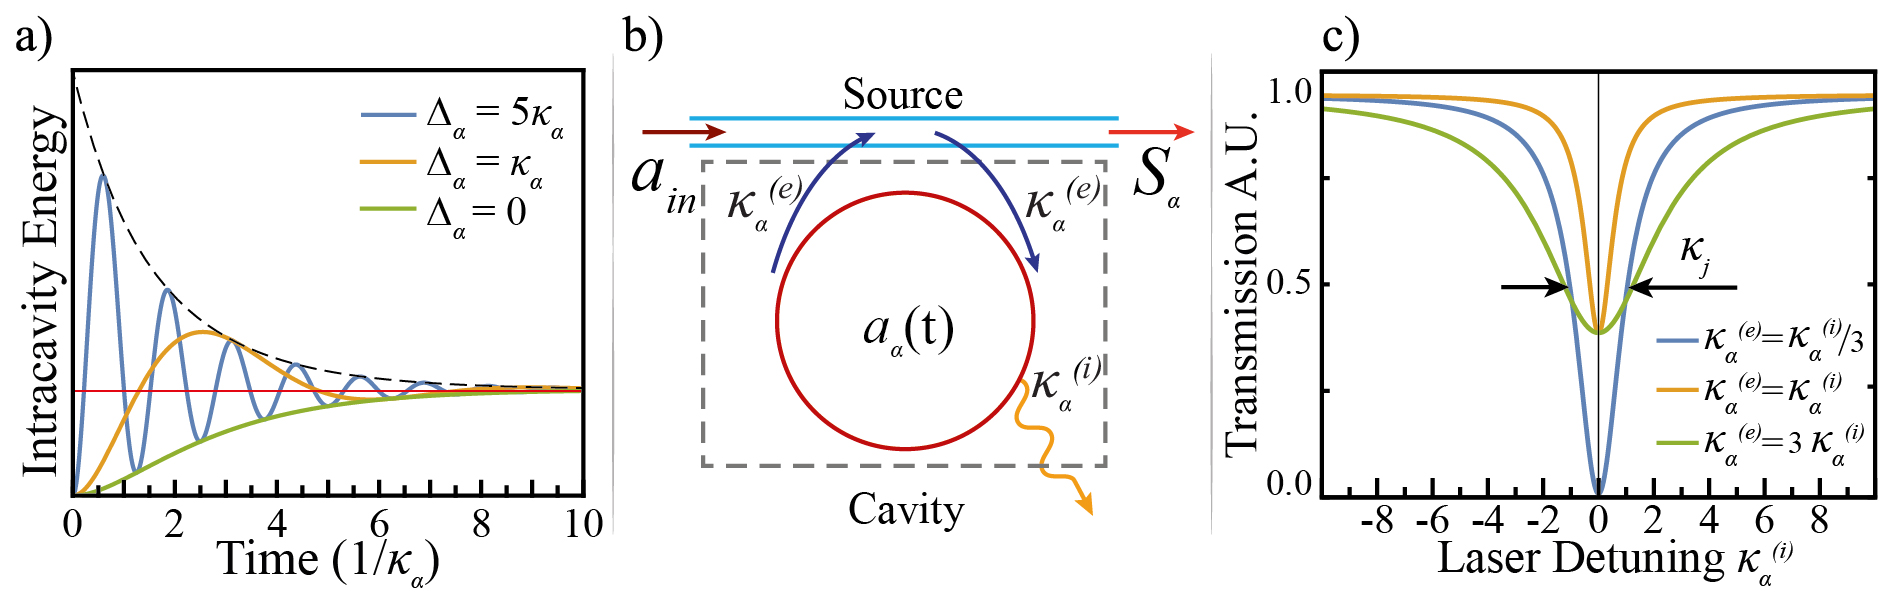
\includegraphics[width = 16cm]{Dissertation_rate_equation.jpg}
    \caption{\textbf{a) Time Dependence Solution of Intracavity Energy:} The energy stored in a cavity oscillate in a frequency $\Delta_\alpha$ and decay with a rate $\kappa_\alpha$ to the Stead Solution. \textbf{b) Picture System:} Our System are compound by a cavity with a single mode $a_\alpha$ that presents intrinsic loss $\kappa_\alpha^{(i)}$. The mode couple with a Source at a rate $\kappa_\alpha^{(e)}$ and interacts with an incoming wave with complex amplitude $a_{in}$. The squared modulus of the output $S_\alpha$ are measured. \textbf{c) Spectroscopy of the $\alpha$th mode:} The transmission of the cavity gives a Lorentzian curve wheres the full width at half maximum correspond to the total loss. This graphic show it for three different regimes.}
    \label{fig:rate_equations_single_mode}
\end{figure}

The Eq~\ref{eq:rate_equation_unperturbed} accepts harmonic solutions with frequency $\Delta_\alpha$. Nevertheless these solutions decay, with a  $\kappa_\alpha/2$ rate, into a steady state solution. We usually operates the system in a time scale much larger than $\kappa^{-1}$, thus we consider just the steady state solution, as show in Fig~\subref{fig:rate_equations_single_mode}{a}

We have already introduced the required formalism to describe our problem, at this point a more pictorial view of it would be very useful. For that we shall use the Fig~\subref{fig:rate_equations_single_mode}{b}. Lets consider our system composed by a optical cavity and a source. This cavity have a optical mode with amplitude $a_\alpha$, and present intrinsic energy loss $\kappa_\alpha^{(i)}$ due scattering and absorption. The source carry a input wave $a_{in}$ at frequency $\omega$ which couple with the cavity at a $\kappa_\alpha^{(e)}$ rate, the optical mode couple back with the source at the same frequency, in such way that this couple is seen as a loss channel. The outgoing wave, defined as $S_\alpha$, carry information about the source and the optical mode, in this way
\begin{equation}
    S_\alpha = a_{in} - \sqrt{2 \kappa_\alpha^{(e)}}a_\alpha.
\end{equation}
For the steady state solution we have $\dot{a} = 0$, which lead us to define the transmission of the cavity as
\begin{equation}
    T = \left|\frac{S_\alpha}{a_{in}}\right|^2 = \frac{\left(\kappa_\alpha^{(i)} -\kappa_\alpha^{(e)}\right)^2 + (2\Delta_\alpha)^2}{\left(\kappa_\alpha^{(i)} +\kappa_\alpha^{(e)}\right)^2 + (2\Delta_\alpha)^2}.
    \label{eq:single_mode_transmission}
\end{equation}

Typically, the experiment are made by sweep the source frequency, hence the detuning. The ration between the intrinsic loss and the coupling loss define the regime of the system; under coupled, for $\kappa_\alpha^{(e)} < \kappa_\alpha^{(i)}$, critical coupled, for $\kappa_\alpha^{(e)} = \kappa_\alpha^{(i)}$, and over coupled, for $\kappa_\alpha^{(e)} > \kappa_\alpha^{(i)}$; the comparison for each regime can be seen in the Fig~\subref{fig:rate_equations_single_mode}{c} 

As the capacity of recycle photons inside the optical cavity is a important feature, we should use a value to determine how efficiently our cavity does it. For this purpose we define the Finesse as the ratio between the mean lifetime of the photon inside the cavity and the round trip time, or in function of measurable parameters 
\begin{equation}
    \mathcal{F} = \frac{\text{Mean Lifetime}}{\text{Round Trip Time}} = \frac{FSR_\alpha}{\kappa_\alpha}.
    \label{eq:finesse}
\end{equation}
Where $FSR_\alpha$ is the Free Spectral Range of the $\alpha$th mode. Then the intracavity power is equal the input power time $\mathcal{F}$.

However, for our system the round trip time and the mean lifetime are coupled, in the sense that we aren't able to increase or decrease the round trip time without affect the mean lifetime, hence we define the Quality factor ($Q$) as the ration between the frequency of the mode ($\omega_\alpha$) and the bandwidth ($\kappa_\alpha$) to determine the efficiency of our cavity to store photons, supposing that the $FSR_\alpha$ are nearly the same. 

In order to better understand the concept of Free Spectral Range and how do it lead us to the round trip time I must develop the spatial treatment of the modes. 
\subsection{Spatial Equations}

Initially lets consider a propagating wave at frequency $\omega$. From the Maxwell's equations it is possible to write
\begin{subequations}
    \begin{alignat}{2}
    &\nabla^2\vec{h}_\alpha+\beta^2n^2\vec{h}_\alpha &&= \nabla(\nabla\cdot\vec{h}_\alpha),\\
    &\nabla^2\vec{e}_\alpha+\beta^2n^2\vec{e}_\alpha &&= \nabla(\nabla\cdot\vec{e}_\alpha).
    \end{alignat}
    \label{eq:wave_eq_full}
\end{subequations}
Here I defined $\beta = \omega/c$, where $c$ is the speed of light in the vacuum. As the medium that we are interested presents uniform refraction index, the right side of the equation are null. 

We shall assume that the solution is a wave that propagate in $z$ direction with the form $e^{ik_\alpha z}$, hence the Eq~\ref{eq:wave_eq_full} can be rewrite as 

\begin{subequations}
    \begin{alignat}{2}
    &\nabla_t^2\vec{h}_\alpha+(\beta^2n^2-k_\alpha^2)\vec{h}_\alpha &&=0,\\
    &\nabla_t^2\vec{e}_\alpha+(\beta^2n^2-k_\alpha^2)\vec{e}_\alpha &&=0.
    \end{alignat}
    \label{eq:wave_eq}
\end{subequations}
Where $\nabla_t^2 = \nabla^2 - \partial^2/\partial z^2$.

\begin{figure}[b!]
    \centering
    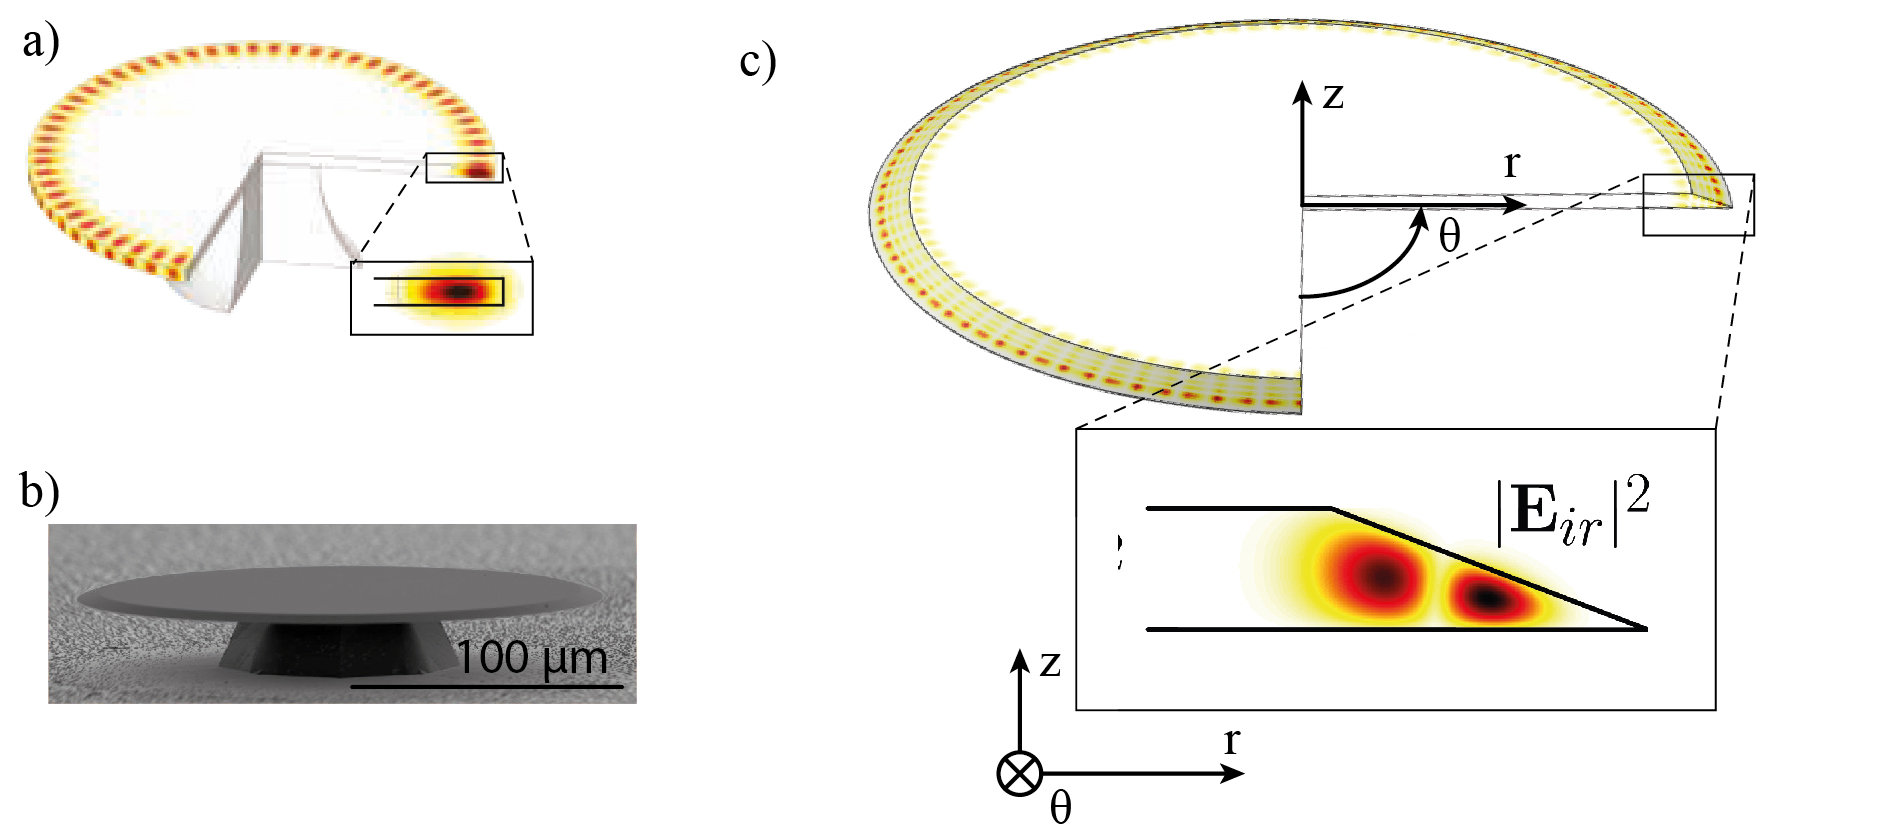
\includegraphics[width =16cm]{Dissertation_wgm.jpg}
    \caption{Caption}
    \label{fig:wgm}
\end{figure}
It might be have been overlooked, but the Eq~\ref{eq:wave_eq} is a system with 6 equation; one for which field in each coordinate. The solution for this set of equation with boundary condition define the optical modes of our problem. To solve this equations we must apply consideration about symmetry, however we use numerical methods to solve it. We will use the commercial software COMSOL\regmark, in Appendix~\ref{app:Comsol_Solution} we explained step by step how this solutions are done. 

Until now we have talk about generic electromagnetic modes, with no spatial boundary condition, in order to define them we must define the geometry of our cavity. Our device are based in disk microcavities, as show in Fig~\subref{fig:wgm}{a}, this kind of resonator presents the so called Whispering Gallery Modes (WGM), due to cylindrical symmetry. In order to archive high life time of the photons inside the cavity we use a wedge cavity. Fig~\subref{fig:wgm}{b} show a photo take using a Scanning Electron Microscope (SEM) of the cavity used in this study, the angle present at edge makes the electric field to be less perpendicular to the surface leading to lower loss due to scattering\needcit. The fabrication process have a important role in here, as we shall see below. 

The boundary condition lead to the characteristic equation in the form 
\begin{equation}
    F(k_r,k_\theta,k_z,\omega) = 0.
    \label{eq:char_eq}
\end{equation}
The solution of this equation in function of the frequency $\omega$ give us the dispersion. 

The set of constants, $k_r,k_\theta,k_z$, that solve this equation define a mode. As the mode is confined in a region, we can correlate this constants, that can assume any complex value, to integer with spatial representation.

The WGM are labeled in the format TExy and TMxy modes, where x and y are integer correlated with $k_r$ and $k_z$, respectively. Beside that, given a TExy (TMxy) mode it can have several values of $m$, which is a integer correlated with $k_\theta$, it also define the family of the mode. The value of x,y and $m$ can be interpreted as the number of antinodes in the intensity of the electric field in each coordinate as defined in the Fig~\subref{fig:wgm}{c}. Just to clarify the nomenclature adopted in this dissertation, henceforward the term '$\alpha$th mode' are applied for a TExy or TMxy mode with any value of $m$. 

The solution of the Eq~\ref{eq:char_eq} give rise to the dispersion of the cavity. As the Round Trip Time depend on the group velocity, it can be extracted from the dispersion by the relation
\begin{equation}
    \text{Round Trip Time} \approx \frac{2\pi R}{v_g} = \frac{2\pi R}{d\omega/dk_\theta} 
\end{equation}

Due to the discretization of the values of $k_\theta$ we can be approached as a differentiation, leading to
\begin{equation}
    \frac{d\omega}{dk_\theta} \approx \frac{\Delta \omega}{\Delta k_\theta} = R\frac{\Delta \omega}{\Delta m}
\end{equation}
The $FSR$ is the linear frequency between two consecutive modes, so
\begin{equation}
    v_g \approx 2\pi R~FSR \Rightarrow \text{Round Trip Time} \approx FSR^{-1} 
\end{equation}

Now we have enough knowledge to understand how to experimentally characterize our devices. The following Section will treat this subject. 

\section{Optical Characterization}

The mainly parameters of relevance to characterize an optical mode is the losses, which is done be measuring the transmission and compare with the Eq~\ref{eq:single_mode_transmission} from the single mode model. 

The experiment is made using the setup showed in the  Fig~\ref{fig:exp_mode_charac}a; A laser with tunable frequency are applied as source, a piezo tunes the size of the external cavity leading to a few GHz of modulation. A small part of the output light are directed to a frequency calibrator compound of a Mach Zehnder interferometer and a wavelength reference Hydrogen Cyanide (HCN) cell. An attenuator control the input power in the cavity. The polarization of the input wave are controlled using a manual fiber polarization control. We use a tapered optical fiber to couple the source with the cavity. The transmission are measured using a power meter and the data are acquired using a DAQ. 
\begin{figure}[h!]
    \centering
    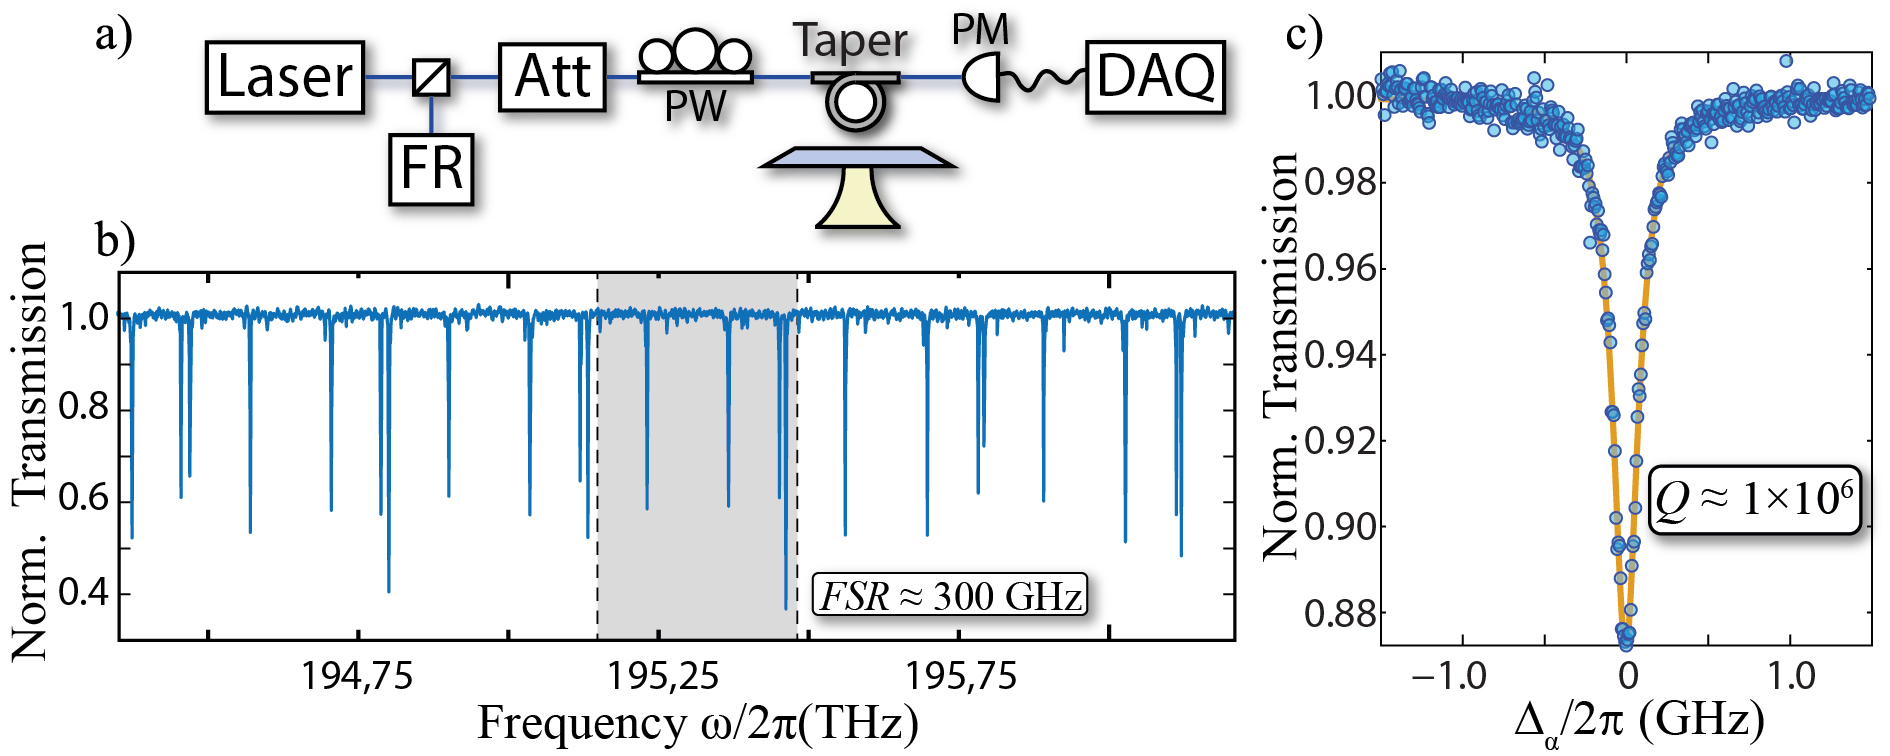
\includegraphics[width = 16cm]{figuras/Dissertation_optical_char_exp.jpg}
    \caption{Caption}
    \label{fig:exp_mode_charac}
\end{figure}

The result, for a single mode, are presented in the Fig~\ref{fig:exp_mode_charac}b). We use the Eq~\ref{eq:single_mode_transmission} to fit the data giving the values of $300$ MHz and $50$ MHz for the $\kappa_\alpha^{(i)}$ and $\kappa_\alpha^{(e)}$, respectively. The mode are at frequency $\omega_\alpha = 2\pi\times195.25$ THz which give us a $Q \approx 2\times10^6$.

Using an stepper motor instead of the piezo it possible to modulate the frequency in few THz enabling us to measure different families of modes, as show in Fig~\ref{fig:exp_mode_charac}c). The spectral distance of a mode in consecutive families give the $FSR_\alpha$ for the $\alpha$ mode. Our cavities present an FSR around $300$ GHz, which have to due mostly with the radius of the device. 

According with the Eq.~\ref{eq:finesse}, we reached a finesse of about $\mathcal{F} \approx 1000$. A device with this parameters enable to amplify the incoming power, due to photons recycling, about $1000$ times. If used a input power of $1$ W, we can reach the $1$ KW of circulating power mentioned at the begin of this Chapter. In general terms, it make our device a good platform to generate nonlinear effects. 

A Fraction of the losses are due the material absorption, when we are working with high intracavity power this absorption lead to a thermal effects called bistability. 

\subsection{Pump Bistability}
The resonance frequency of the cavity are correlated with the refractive index of the material, which is a function of the temperature. Treating this as a perturbation problem, we can write \begin{figure}[b]
    \centering
    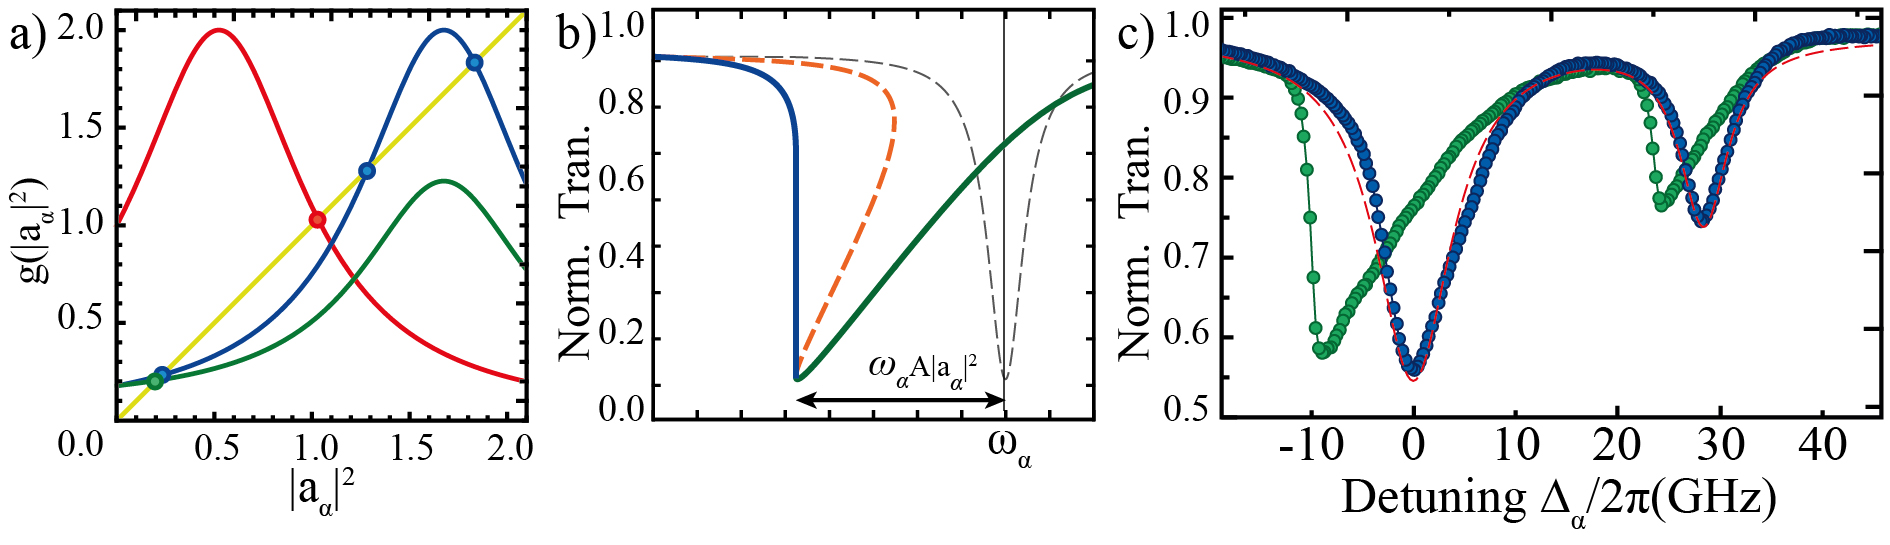
\includegraphics[width = 16cm]{Dissertation_bistabilite.jpg}
    \caption{Caption}
    \label{fig:bistable}
\end{figure}

\begin{subequations}
    \begin{alignat}{2}
        \frac{\Delta\omega_\alpha}{\omega_\alpha} &= -\frac{\Delta \text{n}_\text{eff}}{\text{n}_\text{eff}}\\
        \frac{\Delta\omega_\alpha}{\omega_\alpha} &= -\frac{\int \text{n}^2\vec{e}^*\Delta\text{n}(T)~\vec{e} d^3r}
        {\int \text{n}^2 |\vec{e}|^2 d^3r}
    \end{alignat}
\end{subequations}
Where $T$ are the temperature of the optical mode. In a good approximation, considering a small variation in the temperature, we can write
\begin{equation}
    \Delta \text{n}(T) = \frac{d\text{n}}{dT}\Delta T
\end{equation}
Here, the $\Delta T$ is proportional from the amount of energy absorbed by the material. As we are interested just in the contribution of this effect not in a explicit formula we can suppress all the process of energy conversion in a single constant and write the variation in the frequency in function of the energy storage in the cavity, in such way
\begin{equation}
\frac{\Delta \omega_\alpha}{\omega_\alpha} = A |a_\alpha|^2
\label{eq:pertubation_bistaliti_cavity}
\end{equation}   

Including the contribution in the rate equation, Eq~\ref{eq:rate_equation2}, after the transformation of reference frame, the bistable rate equation can be write as 
\begin{equation}
\dot{a}_\alpha = -\left(i\Delta_\alpha + i\omega_\alpha A|a_\alpha|^2 + \frac{\kappa_\alpha}{2}\right)a_\alpha + \sqrt{\kappa^{(e)}_\alpha}a_{in}
\label{eq:rate_equation_bistable}
\end{equation}

As usual, we looking to the steady state solution. Depending on the $\Delta$ value, this equation can present three different solutions. To visualize it, lets write the Eq~\ref{eq:rate_equation_bistable} as 
\begin{equation}
    |a_\alpha|^2 = \frac{4\kappa^{(e)}_\alpha |a_{in}|^2}{4\left(\Delta_\alpha + \omega_\alpha A|a_\alpha|^2\right)^2+\kappa_\alpha^2} 
\end{equation}

The Fig~\ref{fig:bistable}a
shows the plot of the LHS and RHS in function of $|a_\alpha|^2$. Depending on the value of $\Delta_\alpha$ and $|a_{in}|$ there are three different solutions for this equation, but the intermediate one is always unstable, which lead to the well-know bistable transmission show in Fig~\ref{fig:bistable}b
Controlling the input power using the attenuator, as showed in the setup of the Fig~\ref{fig:exp_mode_charac}c, it is possible to experimental measure the bistability, this measure are show in Fig~\ref{fig:bistable}c 
.

As the pump frequency get closer to the resonance frequency, the intracavity power increases, which shifts the resonance to the red through self-phase modulation, until the pump frequency, $\omega$, reaches the resonance frequency, $\omega_\alpha$; at this point, the effective detuning is zero and the energy stored in the cavity it's maximum.  

As the amplitude is normalize in such way that $|a_\alpha|^2$ is the energy storage in the cavity, hence is proportional to the intensity of the electric field, the effect felt by the cavity due to the Eq~\ref{eq:pertubation_bistaliti_cavity} is similar to the Kerr effect presented in the Eq~\ref{eq:kerr_effect_free_wave}, in fact, in some conditions the both effects are indistinguishable\needcit. For that reason both effects, bistability thermal and Kerr, will all be included in the same term of the rate equation~\ref{eq:rate_equation_bistable}.

The bistability plays an important role in harmonic generation in optical cavity. Further this role will by better understood.  

As mentioned before, the fabrication of the cavity plays a important role in this study. The fallowing Chapter shall treat of the process of fabrication. 
